\documentclass[11pt,a4paper]{article}
\usepackage[utf8]{inputenc}
\usepackage[T1]{fontenc}
\usepackage{lmodern}
\usepackage[margin=2.5cm]{geometry}
\usepackage{amsmath,amssymb,amsthm}
\usepackage{booktabs}
\usepackage{graphicx}
\usepackage{microtype}
\usepackage{xcolor}
\usepackage{url}
\usepackage[numbers,sort&compress]{natbib}
\usepackage[colorlinks=true,linkcolor=blue!50!black,citecolor=blue!50!black,urlcolor=blue!50!black]{hyperref}
\setlength{\parskip}{0.4em}
\setlength{\parindent}{0pt}
\newtheorem{proposition}{Proposition}

\title{Calibrated, Label-Free Screening for Coordinated Manipulation and Best-Response Evaluation of Exchange Rules in a Vietnam-Calibrated Market Simulator}
\author{Quang-Vinh Dang\\
British University Vietnam, Hung Yen, Vietnam\\
\texttt{vinh.dq4@buv.edu.vn} \quad ORCID: 0000-0002-3877-8024}
\date{Draft, October 2026}

\begin{document}
\maketitle

\begin{abstract}
Prosecuted manipulation on the Vietnamese stock exchanges is mostly carried out by groups of accounts that trade in step with each other, yet regulators have no labelled cases to train a detector on and the order-level data needed to test one is not public. We study this problem in an agent-based limit order book calibrated to published rules and to public price data for Vietnam. We propose a coincidence test that asks, for each account and time window, whether its order submissions coincide with those of all other accounts more often than chance, with an exact circular-shift null; netting buys against sells makes market-making desks, which quote both sides at once, neutral. The test needs no labels, and its false-alarm rate is controlled at the nominal level in clean markets (1.1\% of honest accounts at $p\le 0.01$). It finds a colluding ring in the top five accounts of a window in 85--90\% of ring-active windows in a clean simulated market, but only 52\% when honest synchronised groups are present, and its sensitivity falls as the number of accounts grows. A gradient-boosting model trained with labels on simulated rings is more accurate in every scenario, so the test is useful only where labels do not exist. Evaluating rules against a colluding ring that re-optimises its parameters, we find that inspection with a fine proportional to the illegal gain removes most of the ring's expected benefit, that pricing off-book block trades at a trailing mean is the only structural rule with a comparable point estimate, and that the daily price band has no effect. Public prices carry signal for documented cases: a market-adjusted abnormal-return rank places 8 of 10 enforcement cases in the daily top ten of about 1,360 stocks, against 15\% for random stocks, and 701 Telegram-organised pumps show accumulation before the pump that is too weak for early warning. We state clearly what is not established: no real account-level data has been used.
\end{abstract}

\section{Introduction}

A securities regulator that wants to find manipulation faces three problems at once. It rarely has labelled cases, because enforcement is slow and selective. It cannot easily evaluate a rule change before introducing it, because the behaviour of manipulators changes with the rule. And the data that would let an outside researcher test a method, orders tagged with an account, is held only by the exchange and the regulator. These are acute in Vietnam. In ten recent decisions of the State Securities Commission with exact dates (Appendix~\ref{app:cases}) the manipulation was carried out with between 5 and 164 accounts (median 24.5), by trading continuously, or crossing orders among accounts, to create the appearance of supply and demand. Spoofing and layering, the focus of most of the detection literature \citep{tuccella2021,fabre2025}, do not appear among these cases.

We make four contributions. (i)~We state a label-free coincidence test for coordinated accounts and prove that it controls false alarms exactly under a stated exchangeability condition (Section~\ref{sec:method}). (ii)~We measure where it fails: against honest groups that also act in step, such as market-making desks, funds that split orders across sub-accounts and bot fleets reacting to one signal, and as the number of accounts grows (Section~\ref{sec:detect}). (iii)~We evaluate regulatory levers against a colluding ring that re-optimises its parameters, in a simulator calibrated to Vietnamese rules and to public price statistics (Section~\ref{sec:policy}). (iv)~We check what can be checked on real public data: documented enforcement cases against daily prices and a large set of labelled pump events on tick data (Section~\ref{sec:real}).

The paper does not claim that the detector works on real order data. Its manipulators and its features are written by us, a supervised model trained in the simulator does better than the label-free test in every scenario, and the real-data checks are at the level of the stock, not of the account. The contribution is a calibrated screening tool with a measured failure profile, and an evaluation method for rules that does not assume manipulators stand still.

\section{Related work}

\paragraph{Detection of manipulation.} Machine-learning detectors for spoofing and layering work on the order book with labelled or simulated examples \citep{tuccella2021,fabre2025}. Wash trading has been detected by graph rules on exchange data \citep{victor2021}, by dynamic programming on matched orders \citep{cao2016}, and by label-free statistical regularities of reported volume \citep{cong2023}. Collusion among traders has been approached through clustering of trade graphs \citep{palshikar2008} and through degree-strength statistics against randomised networks in Chinese trade data \citep{sun2012}; timing synchrony between traders has been described as a trait of performance rather than of collusion \citep{saavedra2011}, and has been used to build networks of insiders from filings \citep{jaeger2025}. Pump-and-dump schemes organised on messaging channels have been studied with labelled events \citep{xu2019,lamorgia2020,lamorgia2023,hu2022} and priced as a market phenomenon \citep{dhawan2023}. We found no study that applies a time-shift coincidence test to the order submissions of accounts, and no study of account-level collusion with Vietnamese order data; our searches were not exhaustive.

\paragraph{Coincidence tests with surrogates.} Testing whether events in two series coincide more than chance, without a model for the series, is a long-standing problem in neuroscience, where jitter and dither surrogates are used \citep{amarasingham2012,louis2010,grun2009}. Interval jitter gives exact tests, whereas resampling that moves each event about its own position can inflate false positives \citep{platkiewicz2017}. \citet{liang2025} give finite-sample false-positive guarantees for time-shift tests that allow dependence within the series. Our statistic applies that idea to one account against the aggregate of all others, adds the netting of buys and sells, and takes the maximum over tolerances within a single shift distribution.

\paragraph{Simulation for rule design and for evaluating surveillance.} Agent-based markets have been used to test tick size \citep{zhao2020}, price limits \citep{zhang2016} and minimum resting times, cancellation fees, circuit breakers and transaction taxes \citep{leal2019}, using open simulators \citep{byrd2020}; their realism is a recognised issue \citep{vyetrenko2019,platt2018}. The closest work to ours on manipulation is the adversarial framework of \citet{wang2020}, in which a generator learns to evade a discriminator, and the evaluation of a cloaking rule against an adaptive spoofer \citep{wang2018}. We differ by studying a ring rather than a single manipulator, by calibrating to a specific market, and by measuring regulatory levers by the best response of the manipulator. Our treatment of fines follows the economics of enforcement, in which deterrence depends on the product of the probability of detection and the sanction \citep{becker1968,polinsky2000}; double oracle and inspection games are the natural next step \citep{mcmahan2003,lanctot2017,avenhaus2002}. Empirical work on manipulation prevalence \citep{aggarwal2006,comerton2014,khwaja2005} and on Vietnamese markets \citep{nguyen2017,nguyen2023} motivates but does not overlap with our design.

\section{A calibrated simulator}\label{sec:sim}

\paragraph{Market.} A limit order book with price-time priority and self-trade prevention; one step is about one trading minute and a day has 240 steps. Honest agents are noise traders, market makers that re-quote two levels per side and shift with displayed depth imbalance, fundamental traders that follow a noisy latent value, capped momentum traders, depth-imbalance traders, and institutions that slice a parent order into market orders.

\paragraph{Manipulators.} A \emph{ring} of $K$ accounts (3 to 40) runs cycles of accumulation by passive buys, a push by near-simultaneous aggressive buys from several members with some cross trades, and distribution by passive sells of the stock it holds; no member sells short. Orders are spread over members; a jitter parameter spreads the members' actions in time. Outside its campaign each account trades as a noise trader. The ring's benefit is a block held beforehand (3000 lots, an assumption) and sold off-book at the end of each push, valued at the achieved price displacement, plus trading profit. Single-account spoofers, pump-and-dump agents and wash pairs are also implemented.

\paragraph{Honest groups that act in step.} A market-making firm with three to five desks that re-quote together; a fund that splits parent orders across 6 to 12 sub-accounts in the same step; and a fleet of bots that react to one public price signal with small latency differences.

\paragraph{Rules.} The exchange can apply a tick size, minimum resting time, cancel fee, circuit breaker, daily price band, and a reference-price rule for off-book blocks (the last price or a trailing mean).

\paragraph{Calibration to Vietnam.} Prices are in HOSE ticks: a stock at 25,000 VND with a 50 VND tick has a relative tick of 20\,bp, and the daily band is $\pm 7\%$ of the previous close. Rules and statistics come from broker summaries and press (Appendix~\ref{app:calib}); the exchange rulebooks could not be fetched. We add measurements from two public datasets: VN30 and VN-Index bars from 2012, and 1.56 million VN30 futures ticks with best bid and ask from 2024 to April 2025. Table~\ref{tab:calib} compares the preset with these numbers. Cancel share, relative tick and daily volatility are matched; the spread (3 ticks against one tick in 73\% of futures quotes), the tails (excess kurtosis 4--5 daily and 40 at one minute) and volatility clustering are not.

\begin{table}[t]
\centering\small
\begin{tabular}{lrrl}
\toprule
moment & simulator & real & source\\
\midrule
cancel share of orders & 0.321 & 0.318 & HOSE, December 2020 (press)\\
relative tick (bp) & 21 & 20 & derived from the tick table\\
daily volatility (\%) & 1.14 & 1.16 & VN30, 2023 onward\\
retail share of value & 0.72 & 0.75--0.82 & press estimates, 2024--25\\
spread: share of quotes at one tick & 0 & 0.73 & VN30F1M, 2024--25\\
\bottomrule
\end{tabular}
\caption{Calibration of the Vietnam preset. The last row is not matched.}\label{tab:calib}
\end{table}

\section{A calibrated, label-free coincidence test}\label{sec:method}

Take a window of $T$ steps and $n$ accounts. Let $x_i[t]$ be account $i$'s number of buy submissions minus sell submissions at step $t$, and $y_{-i}[t]=\sum_{j\ne i}x_j[t]$. For a tolerance $\tau$ let $\tilde y^{\tau}_{-i}[t]=\sum_{|d|\le\tau}y_{-i}[(t+d)\bmod T]$. For a shift $k\in\{0,\dots,T-1\}$ define
\begin{equation}
C^{\tau}_i(k)=\sum_{t}x_i[(t-k)\bmod T]\;\tilde y^{\tau}_{-i}[t],\qquad
Z_i(k)=\max_{\tau\in\mathcal T}\frac{C^{\tau}_i(k)-\bar C^{\tau}_i}{s^{\tau}_i},
\end{equation}
where $\bar C^{\tau}_i$ and $s^{\tau}_i$ are the mean and standard deviation of $C^{\tau}_i(k)$ over $k$. The statistic is large when the account submits on the same side as the others at the same moments. The observed value is $Z_i(0)$ and the $p$-value is
\begin{equation}
p_i=\frac1T\,\#\{k:\,Z_i(k)\ge Z_i(0)\}\in[1/T,1].
\end{equation}
All $T$ shifts are computed by fast Fourier transform, so a window of $n$ accounts costs $O(nT\log T)$ per tolerance. The default is $T=300$ and $\mathcal T=\{1,5,15\}$. The unsigned variant keeps buys and sells as two channels and sums their statistics.

\begin{proposition}\label{prop:exact}
Suppose that under the null hypothesis the pair $(x_i,y_{-i})$ is invariant in law to a cyclic shift of $x_i$ alone, that is, $(g\,x_i,\,y_{-i})\overset{d}{=}(x_i,\,y_{-i})$ for every cyclic shift $g$. Then $\Pr(p_i\le\alpha)\le\alpha$ for every $\alpha\in[0,1]$.
\end{proposition}
\begin{proof}
Write $Z_k=Z_i(k)$ and $R_m=\#\{k: Z_k\ge Z_m\}$. Since $Z_k(x,y)=Z_0(g^k x,y)$, we have $R_m(x,y)=R_0(g^m x,y)$, and by invariance $R_0\overset{d}{=}R_m$ for every $m$. For any real vector $(Z_k)$, at most $\lfloor\alpha T\rfloor$ indices $m$ satisfy $R_m\le\alpha T$. Hence $\Pr(R_0\le\alpha T)=\tfrac1T\sum_m\Pr(R_m\le\alpha T)=\tfrac1T\mathbb E\,\#\{m:R_m\le\alpha T\}\le\alpha$. \qedhere
\end{proof}

The maximum over tolerances is taken inside $Z_i(k)$ for the same $k$, so it does not break the argument. The proposition is the standard randomisation-test argument; \citet{liang2025} treat the dependence within the series that makes it applicable to real time series. Its condition is strong. It fails when an account's activity and the others' activity share a trend inside the window, and when honest accounts respond to the same events; honest groups that act in step are precisely a violation, which is why we measure the false-alarm rate empirically (Section~\ref{sec:detect}). Netting buys against sells before testing makes accounts that quote both sides at the same moment contribute nothing, while one-directional coordination does not cancel.

The test is used for screening. In each window the $B$ accounts with the highest $Z_i(0)$ are the ones inspected, or accounts with $p_i\le\alpha$ are flagged. A ring is \emph{caught} if one member is inspected in some window, on the assumption that finding one member exposes the others, as account linking does in practice.

\section{Detection experiments}\label{sec:detect}

All numbers in this section are for the default simulator (about 120 accounts in a window), one ring per episode, and episodes of 6000 steps (19 windows of 300 steps). Metric: \emph{catch@$B$}, the share of ring-active windows in which one of the $B$ top-ranked accounts is a ring member, with 95\% bootstrap intervals over 24 test episodes.

\paragraph{Calibration.} In a market without rings, 1.1\% of honest accounts have $p\le 0.01$ (market makers 0.7\%, momentum traders 2.7\%), in line with the nominal rate.

\paragraph{Robustness to honest synchronised groups.} Table~\ref{tab:robust} and Figure~\ref{fig:robust} give catch@5 with and without honest groups. The three baselines that need no labels fail on the ring: the order-to-trade ratio is dominated by market makers, which sit far above manipulators, and an isolation forest on account features finds almost nothing. The unsigned test finds the ring in a clean market but collapses when market-making desks are present, because the desks, which quote both sides at once, are flagged at 71\% (Table~\ref{tab:groups}) and fill the top of the ranking. Netting buys against sells removes the effect of the desks (the desks' flag rate falls to 0 in that scenario). A fund that splits orders across sub-accounts is genuinely coordinated and is flagged at 6\% whatever the variant; it reduces catch@5 to 0.74. With all three groups together catch@5 is 0.52 for the signed test and 0.23 for the unsigned one. A gradient-boosting model trained with labels on rings in the clean market stays at 0.98--1.00 in every scenario.

\begin{figure}[t]
\centering
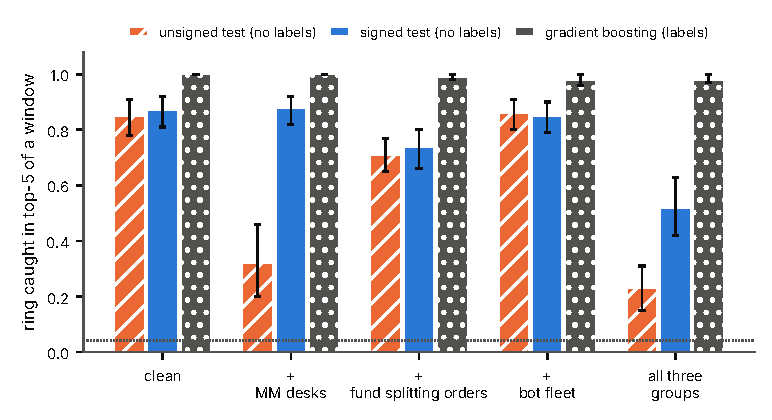
\includegraphics[width=0.85\linewidth]{figures/robust.pdf}
\caption{Share of ring-active windows in which a ring member is among the five top-ranked accounts, with 95\% bootstrap intervals over 24 episodes. The dotted line is the chance level. The unsigned test is crowded out by market-making desks; the signed test is not. Gradient boosting is trained with labels on rings in the clean market.}\label{fig:robust}
\end{figure}

\begin{table}[t]
\centering\small
\begin{tabular}{lccccc}
\toprule
detector & clean & +MM desks & +fund splitting orders & +bot fleet & all three \\
\midrule
order-to-trade ratio & 0.00\,{\scriptsize[0.00, 0.00]} & 0.00\,{\scriptsize[0.00, 0.00]} & 0.00\,{\scriptsize[0.00, 0.00]} & 0.13\,{\scriptsize[0.05, 0.22]} & 0.09\,{\scriptsize[0.04, 0.14]} \\
isolation forest (no labels) & 0.01\,{\scriptsize[0.00, 0.02]} & 0.01\,{\scriptsize[0.00, 0.02]} & 0.00\,{\scriptsize[0.00, 0.00]} & 0.01\,{\scriptsize[0.00, 0.03]} & 0.02\,{\scriptsize[0.00, 0.03]} \\
coincidence test, unsigned (no labels) & 0.85\,{\scriptsize[0.78, 0.91]} & 0.32\,{\scriptsize[0.20, 0.46]} & 0.71\,{\scriptsize[0.65, 0.77]} & 0.86\,{\scriptsize[0.80, 0.91]} & 0.23\,{\scriptsize[0.15, 0.31]} \\
coincidence test, signed (no labels) & 0.87\,{\scriptsize[0.81, 0.92]} & 0.88\,{\scriptsize[0.82, 0.92]} & 0.74\,{\scriptsize[0.66, 0.80]} & 0.85\,{\scriptsize[0.79, 0.90]} & 0.52\,{\scriptsize[0.42, 0.63]} \\
gradient boosting (labels, clean market) & 1.00\,{\scriptsize[1.00, 1.00]} & 1.00\,{\scriptsize[1.00, 1.00]} & 0.99\,{\scriptsize[0.98, 1.00]} & 0.98\,{\scriptsize[0.96, 1.00]} & 0.98\,{\scriptsize[0.97, 1.00]} \\
\bottomrule
\end{tabular}

\caption{catch@5 in a clean market and with honest groups acting in step (95\% bootstrap intervals).}\label{tab:robust}
\end{table}

\begin{table}[t]
\centering\small
\begin{tabular}{llrrr}
\toprule
scenario & honest group & members scored & flagged, unsigned & flagged, signed\\
\midrule
+ MM desks & market-making desks & 2622 & 0.711 & 0.000\\
+ fund splitting orders & fund sub-accounts & 5277 & 0.061 & 0.063\\
+ bot fleet & bot fleet & 3571 & 0.013 & 0.016\\
all three & market-making desks & 2698 & 0.665 & 0.182\\
all three & fund sub-accounts & 5202 & 0.050 & 0.053\\
all three & bot fleet & 3732 & 0.029 & 0.037\\
\bottomrule
\end{tabular}
\caption{Honest group members flagged at $p\le 0.01$ (nominal 1\%).}\label{tab:groups}
\end{table}

\paragraph{Sensitivity.} Figure~\ref{fig:sens} and Table~\ref{tab:ablation} (Appendix) vary the design. The tolerance set and the window length matter little (catch@5 between 0.88 and 0.91). Sensitivity falls with the number of accounts: from 0.91 with 100 accounts to 0.84, 0.64 and 0.28 with 206, 373 and 708. It rises with ring size (0.79 for four accounts, 0.94 for 16 or more) and with the ring's activity (0.46, 0.79, 0.91 for push probabilities 0.2, 0.4, 0.8). The dependence on the number of accounts is the main weakness of ranking by top-$B$; a rule based on the $p$-value and a false-discovery-rate bound would scale differently, and we have not tested it.

\begin{figure}[t]
\centering
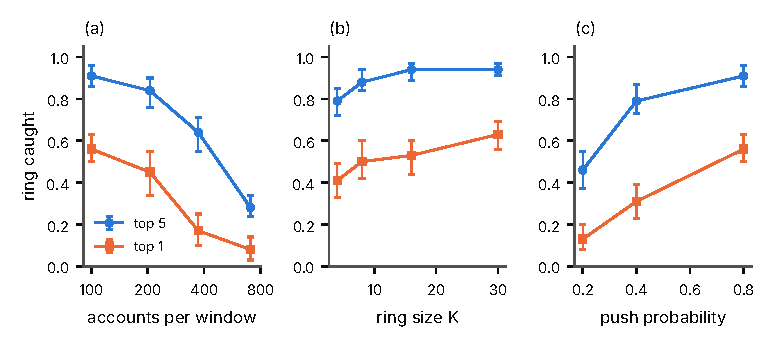
\includegraphics[width=\linewidth]{figures/sensitivity.pdf}
\caption{Sensitivity of the signed test in a clean market: (a) number of accounts per window, (b) ring size, (c) push probability of the ring. Bars are 95\% bootstrap intervals over 16 episodes.}\label{fig:sens}
\end{figure}

\paragraph{What the label-free test is for.} The model trained with labels is better in every scenario. The test is useful when there are no labels, which is the regulator's position, and when one cannot trust that a model trained on simulated rings transfers to real ones. We cannot say which of the two would do better on real data.

\section{Evaluating rules against a ring that adapts}\label{sec:policy}

\paragraph{Design.} The ring chooses its parameters (size, order size, members per push, push and accumulation probabilities, timing jitter, cross-trade share, phase lengths, cool-down) to maximise its net benefit $U=g-m\max(g,0)\,\mathbb 1[\text{caught}]$, where $g$ is its gain and $m$ the multiple of the illegal gain that the fine represents; Vietnamese administrative fines are capped at five times the gain for individuals and ten times for organisations (Appendix~\ref{app:calib}). With a fine of $m$ times the gain, deterrence requires a probability of detection above $1/m$ \citep{becker1968}. The search is an evolution strategy with common random numbers; because single runs were noisy and non-monotone across policies, every policy faces the same set of seven strategies found anywhere, the ring picks the best on 20 selection episodes, and the table reports 20 separate episodes. The result is a lower bound on a fully adaptive ring's benefit. The market is the Vietnam preset (about 580 active accounts per window).

\paragraph{Results.} Table~\ref{tab:policy} and Figure~\ref{fig:policy} show the outcome. (i)~The daily price band is not binding: the ring moves the price by about 0.5\% against a band of 7\%, and widening the band to 10\% or 15\%, which the securities commission is studying, changes nothing. (ii)~Inspecting one or three accounts per window with the signed test cuts the ring's best gain by about 83\% and makes the expected net benefit negative at both fines; the probability of being caught is 20\% and 45\%, with 0.2--0.5\% of accounts inspected. (iii)~Pricing off-book blocks at the trailing mean of the last 60 or 240 steps cuts the gain by 73\% and 93\% at the point estimate, which is 1.4 and 2 standard errors from the baseline, at a cost to honest block trades of 0.17\% and 0.50\% of the price (the mean gap between the last price and the trailing mean). The remaining gain under the 240-step rule comes almost entirely from trading profit, since the displacement is 0.6 tick.

\begin{figure}[t]
\centering
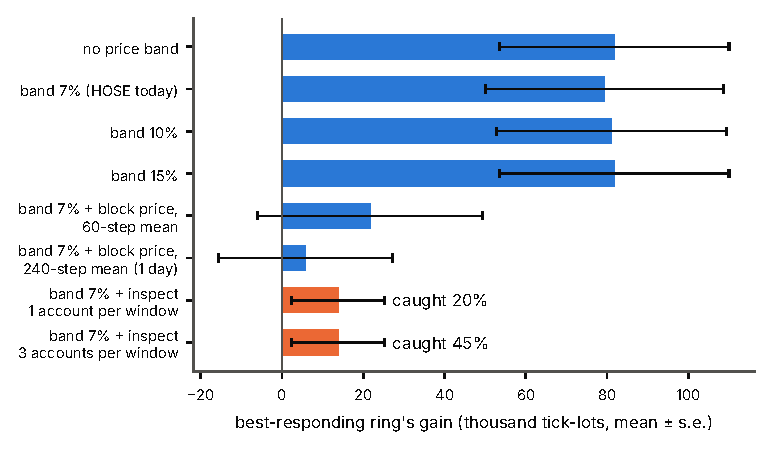
\includegraphics[width=0.85\linewidth]{figures/policy.pdf}
\caption{Gain of the best-responding ring under each policy (thousand tick-lots, mean and standard error over 20 episodes) in the Vietnam preset.}\label{fig:policy}
\end{figure}

\begin{table}[t]
\centering\small
\begin{tabular}{lrrrr}
\toprule
policy & ring gain (mean, s.e.) & caught & net benefit after fine, $m=5$ & $m=10$ \\
\midrule
no price band & 81.7k (28.3k) & -- & -- & -- \\
band 7\% (HOSE today) & 79.4k (29.3k) & -- & -- & -- \\
band 10\% & 81.1k (28.2k) & -- & -- & -- \\
band 15\% & 81.7k (28.3k) & -- & -- & -- \\
band 7\% + block at 60-step mean & 21.7k (27.6k) & -- & -- & -- \\
band 7\% + block at 240-step mean & 5.8k (21.4k) & -- & -- & -- \\
band 7\% + inspect 1 per window & 13.8k (11.4k) & 20\% & -35.6k & -85.1k \\
band 7\% + inspect 3 per window & 13.8k (11.4k) & 45\% & -48.9k & -111.6k \\
\bottomrule
\end{tabular}

\caption{Best-responding ring against each policy. Net benefit is the gain minus $m$ times the gain when caught, with fines of $m=5$ and $m=10$ times the gain.}\label{tab:policy}
\end{table}

\paragraph{Order-level rules against a fixed spoofer.} For the default spoofer, which does not adapt, a minimum resting time of 5 steps removes most of its profit at small cost to market quality, while a tick four times larger widens the spread by 124\% and raises volatility by 50\% without stopping it, and a cancel fee of two raises retail trading cost by 36\% without reducing the spoofing impact (Appendix, Table~\ref{tab:order}). Because the spoofer does not adapt, these effects are upper bounds; we did not compute best responses for spoofing.

\paragraph{Sensitivity to the market.} In the first version of the Vietnam preset, whose daily volatility was 0.4\%, the ring's prize was ten times larger and the block-price rule looked weak; the ranking of levers depends on the market's volatility. We therefore report the calibrated preset only, and we have not repeated the comparison over a family of calibrated markets.

\section{Checks on real public data}\label{sec:real}

\subsection{Documented enforcement cases on daily prices}

\paragraph{Data and protocol.} The price panel holds daily open, high, low, close and volume for 1,551 Vietnamese stocks from 2015 to September 2025 (public data, Appendix~\ref{app:calib}). Ten decisions of the State Securities Commission with exact dates of the conduct were collected from press reports quoting the decisions (Appendix~\ref{app:cases}; the decision documents were not opened). For every stock and date, using only data up to that date, we compute market-adjusted abnormal return, volume surge against the stock's own history, a round-trip statistic, the position of the close in the daily range, the count of days with moves of at least 6.5\%, and range expansion; stocks are ranked against each other on each date. The protocol, fixed before the cases were scored, is: a case stock is scored by the highest rank it reaches on any date in its period; the null is the same statistic for 300 random stocks over the same dates; and we count the cases in which the stock is among the $B$ highest of its date at least once.

\paragraph{Results.} Table~\ref{tab:cases} gives the results. The market-adjusted abnormal return alone places 8 of the 10 cases in the daily top ten of about 1,360 scored stocks at some point of their period, against 15\% for random stocks over the same dates. Combining six features, or using an isolation forest on them, is no better than that single feature, and volume surge is uninformative: these stocks were pushed up on ordinary volume (one stock rose five-fold at 1.02 times its usual volume). We therefore claim nothing new for the market-level detector. The result says little about precision: periods are long (83 to 587 trading days), only ten cases are documented among thousands of price run-ups, and an unlabelled run-up is not an innocent one.

\begin{table}[t]
\centering\small
\begin{tabular}{lrrrrrrr}
\toprule
detector & superiority & top 10 & chance & top 20 & chance & top 50 & chance \\
\midrule
market-adjusted abnormal return & 0.89 & 8/10 & 15\% & 10/10 & 27\% & 10/10 & 53\% \\
combined six-feature score & 0.78 & 6/10 & 22\% & 6/10 & 35\% & 10/10 & 58\% \\
isolation forest, same features & 0.78 & 7/10 & 21\% & 8/10 & 34\% & 9/10 & 54\% \\
round trip (run-up, retracement) & 0.70 & 9/10 & 76\% & 10/10 & 81\% & 10/10 & 90\% \\
volume surge & 0.33 & 0/10 & 3\% & 0/10 & 5\% & 0/10 & 13\% \\
\bottomrule
\end{tabular}

\caption{Ten documented cases scored against about 1,360 stocks. Superiority is the probability that a case stock beats a random stock (0.5 is chance); ``top $B$'' counts cases in which the stock reached the daily top-$B$ list at some date of its period; ``chance'' is the same share for random stocks.}\label{tab:cases}
\end{table}

\subsection{Telegram-organised pump events on tick data}

We use a public archive of 701 pump events with trades from about 24 hours before the pump time to shortly after (Appendix~\ref{app:calib}). The files hold side, price and amount, with no account identifiers, so the coincidence test cannot be applied. For each event, standardised volume and buy imbalance over rolling ten-minute windows are measured against the same coin's first 20 hours. Figure~\ref{fig:pump} shows accumulation: mean standardised volume rises from 0.19 (4 to 3 hours before) to 0.71 (last ten minutes), and buy imbalance from 0.03 to 0.23, with intervals excluding zero, and both jump at the pump. This supports the accumulate--push structure of the simulated ring. It does not give early warning: with the alarm rate in the background set to 0.05 per coin-hour, only 6.0\% of events raise an alarm in the last hour before the pump (8.3\% at 0.1 and 16.4\% at 0.25 per coin-hour; median lead 7 to 15 minutes when it fires).

\begin{figure}[t]
\centering
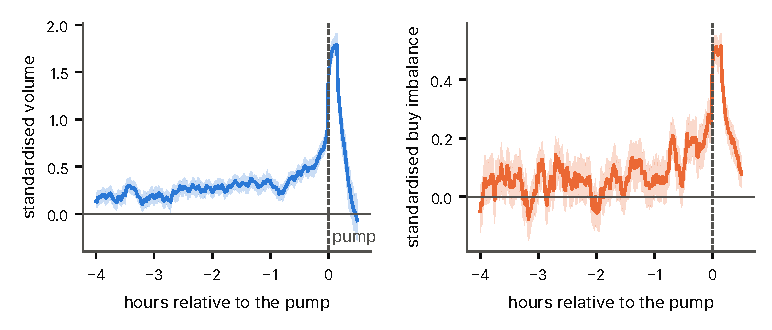
\includegraphics[width=0.85\linewidth]{figures/pump.pdf}
\caption{Standardised volume and buy imbalance of 701 pump events around the pump time (mean and 95\% bootstrap interval over events).}\label{fig:pump}
\end{figure}

\section{Discussion and limitations}

\paragraph{What the evidence supports.} The coincidence test has controlled false alarms and a measured failure profile in the simulator, and netting buys against sells removes one specific and important failure. Inspection with a detector and a fine proportional to the gain is the lever that removes the ring's benefit in the simulator; the price band does not matter for this kind of manipulation; pricing off-book blocks at a trailing mean is a candidate that needs confirmation. On real public prices, a simple abnormal-return rank flags documented cases far above chance.

\paragraph{What it does not support.} No real account-level data has been used, so we do not know whether real rings are separable from honest coordination by this test; the simulator's manipulators and honest groups were written by the same author as the detectors. The Vietnam preset does not reproduce the spread, the tails or volatility clustering. Rule facts come from broker summaries and press. The ring search has a small budget and the standard errors in Table~\ref{tab:policy} are 20\% to 100\% of the means, so only the larger differences are distinguishable from noise; the block value is an assumption, and a ring that is caught is assumed to be exposed by one inspected member. Sensitivity to the number of accounts was measured with different adversaries in different sections. The real-data checks are at the level of the stock, not of the account; the case periods come from press reports; the panel holds only stocks that are still listed.

\paragraph{Next steps.} Account-level data from an exchange, or per-account trade tables from case files, would allow a direct test; a rule based on $p$-values and a false-discovery-rate bound should replace top-$B$ ranking; the interplay of an adaptive ring with an adaptive regulator is a game that double-oracle methods could solve; and the policy comparison should be repeated over a family of markets that all match the published moments.

\section*{Data and code availability}
Code, simulator, experiment scripts, result tables and the case list are in the repository \url{https://github.com/vinhqdang/quantitative_trading}. The public datasets used are listed in Appendix~\ref{app:calib}; raw files are not redistributed.

\section*{Ethics declaration}
The study uses simulated data and public market data; no human subjects were involved. Enforcement cases are identified by stock ticker only; persons named in decisions are not named here.

\section*{Author contributions, funding, conflicts of interest}
\textit{[To be completed by the author: CRediT contribution statement, funding statement, competing-interests statement.]}

\appendix
\section{Documented cases used in Section~\ref{sec:real}}\label{app:cases}
\begin{table}[h]
\centering\footnotesize
\begin{tabular}{llrll}
\toprule
ticker & period & accounts & decided & type \\
\midrule
FIR & 2022-01-04 to 2022-06-17 & 76 & SSC 2023-11 and 2024-01 & cross trading among own accounts \\
SJS & 2023-04-10 to 2024-01-10 & 26 & SSC 2026-01-08 & continuous buying and selling \\
PDR & 2022-08-15 to 2022-12-09 & 164 & SSC 2025-03-21 & cross trading among own accounts \\
PSH & 2021-02-01 to 2022-05-27 & 26 & SSC 2024-05-27 & negotiated trades within a group \\
AGG & 2020-12-01 to 2022-12-31 & 92 & SSC 2025-09 (year inferred) & continuous buying and selling \\
PPT & 2022-06-17 to 2024-10-17 & 19 & SSC decision 881 & continuous buying and selling \\
CRC & 2025-03-03 to 2025-08-01 & 10 & SSC 2025-12-22 & cross trading \\
GKM & 2021-08-02 to 2022-01-28 & 23 & SSC 2023-12-21 & fake supply and demand to push the price up \\
PAS & 2021-01-04 to 2022-12-30 & 19 & SSC 2026-02-12 & continuous buying and selling \\
HCI & 2019-12-13 to 2020-07-16 & 5 & SSC 2024-05-30 & cross matched orders among own accounts \\
HNG & 2015-07-20 to 2016-04-01 & 42 & SSC 2017-08-10 & multi-account fake supply and demand \\
\bottomrule
\end{tabular}

\caption{Cases with exact dates of the conduct. The periods are from press reports quoting the State Securities Commission decisions (sources are listed in the repository file \texttt{data/cases.csv}); the decision documents were not opened. FIR was the subject of two decisions with the same period and is counted once. PSH was traded on the negotiated system.}
\end{table}

\section{Sources for the calibration and real-data checks}\label{app:calib}
\begin{itemize}\itemsep0pt
\item Tick sizes, daily bands, lot sizes, sessions: broker rule summaries (FPTS for HOSE, a securities-company PDF for HNX); the KRX system went live on 5 May 2025. Details and confidence tags: \texttt{docs/vietnam\_calibration.md} in the repository.
\item Fine cap of five times (individuals) and ten times (organisations) the illegal gain: Vietnamese press and legal-news summaries of Decree 156/2020 as amended; not read from the decree.
\item Cancel and amendment share of 31.76\% of orders (December 2020): press report of a HOSE statement.
\item VN30, VN-Index and VN100 bars and the VN30F1M ticks: public Kaggle datasets (keithvo/vnstockdata, khimduong/vn30-market-making).
\item Daily prices of 1,551 stocks: public Kaggle dataset (vuthinh/vietnam-stock-market-ohlc-price-data).
\item Pump events: public Hugging Face dataset (Go3x3/pump\_and\_dump\_dataset, MIT licence).
\end{itemize}

\section{Additional tables}
\begin{table}[h]
\centering\footnotesize
\begin{tabular}{llcccr}
\toprule
factor & level & catch@5 & catch@1 & honest flagged & accounts per window \\
\midrule
tolerances & (1,) & 0.89\,{\scriptsize[0.85, 0.94]} & 0.44\,{\scriptsize[0.38, 0.52]} & 0.013 & 100 \\
 & (1, 5) & 0.88\,{\scriptsize[0.83, 0.93]} & 0.55\,{\scriptsize[0.48, 0.62]} & 0.013 & 100 \\
 & (1, 5, 15) & 0.91\,{\scriptsize[0.86, 0.96]} & 0.56\,{\scriptsize[0.50, 0.63]} & 0.014 & 100 \\
 & (1, 5, 15, 30) & 0.90\,{\scriptsize[0.86, 0.95]} & 0.55\,{\scriptsize[0.49, 0.61]} & 0.014 & 100 \\
window length (steps) & 150 & 0.88\,{\scriptsize[0.83, 0.91]} & 0.41\,{\scriptsize[0.34, 0.47]} & 0.007 & 81 \\
 & 300 & 0.91\,{\scriptsize[0.86, 0.96]} & 0.56\,{\scriptsize[0.50, 0.63]} & 0.014 & 100 \\
 & 600 & 0.91\,{\scriptsize[0.84, 0.97]} & 0.58\,{\scriptsize[0.46, 0.71]} & 0.018 & 108 \\
noise traders (accounts) & 80 & 0.91\,{\scriptsize[0.86, 0.96]} & 0.56\,{\scriptsize[0.50, 0.63]} & 0.014 & 100 \\
 & 200 & 0.84\,{\scriptsize[0.76, 0.90]} & 0.45\,{\scriptsize[0.34, 0.55]} & 0.010 & 206 \\
 & 400 & 0.64\,{\scriptsize[0.55, 0.71]} & 0.17\,{\scriptsize[0.10, 0.25]} & 0.009 & 373 \\
 & 800 & 0.28\,{\scriptsize[0.24, 0.34]} & 0.08\,{\scriptsize[0.03, 0.14]} & 0.010 & 708 \\
ring size K & 4 & 0.79\,{\scriptsize[0.72, 0.85]} & 0.41\,{\scriptsize[0.33, 0.49]} & 0.013 & 93 \\
 & 8 & 0.88\,{\scriptsize[0.84, 0.94]} & 0.50\,{\scriptsize[0.42, 0.60]} & 0.012 & 97 \\
 & 16 & 0.94\,{\scriptsize[0.89, 0.97]} & 0.53\,{\scriptsize[0.44, 0.60]} & 0.012 & 104 \\
 & 30 & 0.94\,{\scriptsize[0.91, 0.97]} & 0.63\,{\scriptsize[0.56, 0.69]} & 0.012 & 115 \\
ring push probability & 0.2 & 0.46\,{\scriptsize[0.37, 0.55]} & 0.13\,{\scriptsize[0.08, 0.20]} & 0.012 & 100 \\
 & 0.4 & 0.79\,{\scriptsize[0.73, 0.87]} & 0.31\,{\scriptsize[0.23, 0.39]} & 0.014 & 100 \\
 & 0.8 & 0.91\,{\scriptsize[0.86, 0.96]} & 0.56\,{\scriptsize[0.50, 0.63]} & 0.014 & 100 \\
\bottomrule
\end{tabular}

\caption{Ablations and sensitivity of the signed test in a clean market (16 episodes per row, 95\% bootstrap intervals). ``Honest flagged'' is the share of honest accounts with $p\le0.01$.}\label{tab:ablation}
\end{table}

\begin{table}[h]
\centering\footnotesize
\begin{tabular}{lrrrrr}
\toprule
policy & spread & volatility & retail cost & spoofing impact & spoofing profit\\
\midrule
baseline & 2.6 ticks & 0.21 & 2.2 & 1.07 & 56\\
tick $\times4$ & $+124\%$ & $+50\%$ & $-54\%$ & $-25\%$ & 687\\
min.\ rest 5 steps & $0\%$ & $-4\%$ & $+11\%$ & $+1\%$ & 13\\
min.\ rest 15 steps & $+3\%$ & $+4\%$ & $+16\%$ & $-17\%$ & $-346$\\
cancel fee 2 & $+1\%$ & $-1\%$ & $+36\%$ & $-5\%$ & 128\\
circuit breaker (6 ticks) & $+1\%$ & $+2\%$ & $-6\%$ & $+3\%$ & 43\\
\bottomrule
\end{tabular}
\caption{Order-level rules against the default (non-adaptive) spoofer, 16 episodes per policy; changes relative to the baseline. Retail cost includes fees paid and falls under larger ticks because simulated noise traders mostly post passive orders and earn the wider spread.}\label{tab:order}
\end{table}

\bibliographystyle{plainnat}
\bibliography{references}

\end{document}
